\documentclass[a4paper, 12pt, final, garamond]{book}
\usepackage{cours-preambule}

\raggedbottom

\makeatletter
\renewcommand{\@chapapp}{\'Electrocin\'etique -- chapitre}
\makeatother

% \toggletrue{student}
% \HideSolutionstrue
% \toggletrue{corrige}

\begin{document}
\setcounter{chapter}{4}

\chapter{\cswitch{Correction du TD}{TD~: circuits \'electriques en RSF}}
% TODO: Refaire toutes les figures.
\resetQ
\section{Impédance équivalente}
\iftoggle{student}{ % pour version student
	\iftoggle{corrige}{ % version avec corrigé : affiche juste la correction
		\begin{enumerate}
			\item On commence par convertir le circuit avec les impédances complexes~:
			      \begin{itemize}
				      \item $\Zu_{C_1} = \frac{1}{\jj C_1\w}$~;
				      \item $\Zu_L = \jj L\w$~;
				      \item $\Zu_{C_2} = \frac{1}{\jj C_2\w}$.
			      \end{itemize}
			      On peut ensuite déterminer l'impédance équivalente à l'association en
			      parallèle de $L$ et $C_2$. Avec les admittances, on a
			      \begin{gather*}
				      \Zu\ind{eq,1}
				      = \frac{1}{\frac{1}{\Zu_{C_2}} + \frac{1}{\Zu_L}}
				      = \frac{1}{\jj C_2\w + \frac{1}{\jj L\w}}
				      = \frac{\jj L\w}{1 - \w^2LC_2}
			      \end{gather*}
			      Il suffit alors de faire l'association en série de $\Zu_{C_1}$ et de
			      $\Zu\ind{eq,1}$~:
			      \begin{gather*}
				      \boxed{
					      \Zu\ind{eq} = \frac{1}{\jj C_1\w} + \frac{\jj L\w}{1 - \w^2LC_2}}
			      \end{gather*}
			      Il n'est ici pas nécessaire d'aller plus loin dans le calcul.

			\item Ici, on utilise que $\Zu_R = R$ et comme précédemment, on effectue
			      l'association en parallèle des $R$ et $C$ de droite avant de faire
			      l'association en série de $R$ et $C$ de gauche avec cette impédance
			      équivalente~:
			      \begin{gather*}
				      \Zu\ind{eq, 1}
				      = \frac{1}{\frac{1}{\Zu_1} + \frac{1}{\Zu_C}}
				      = \frac{1}{\frac{1}{R} + \jj C\w}
				      = \frac{R}{1 + \jrcw}
			      \end{gather*}
			      Et on a donc finalement
			      \begin{gather*}
				      \boxed{
					      \Zu\ind{eq} = R + \frac{1}{\jj C\w} + \frac{R}{1 + \jrcw}}
			      \end{gather*}
		\end{enumerate}
	}{ % énoncé
		Déterminer l'impédance complexe équivalente de chacun des dipôles ci-dessous
		en RSF.
		\begin{center}
			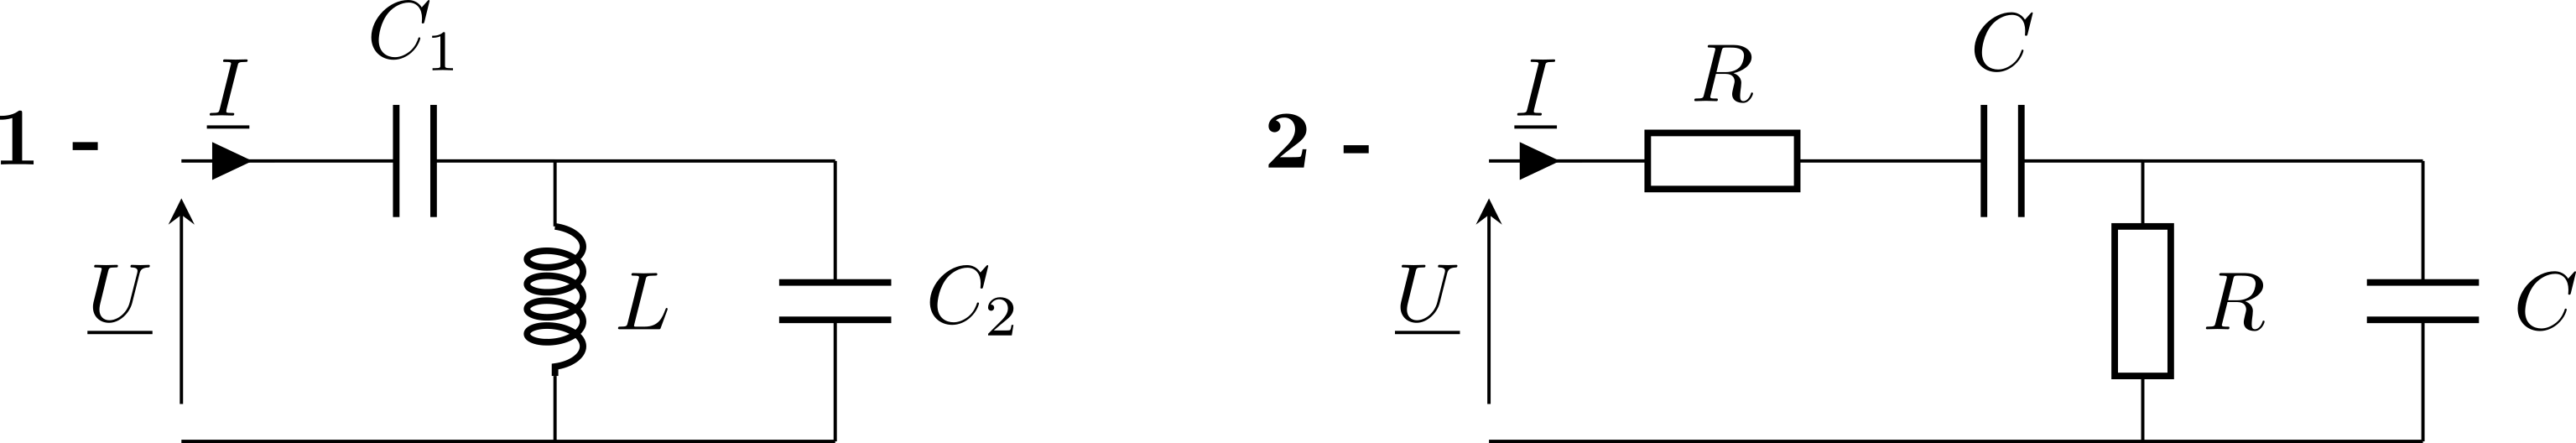
\includegraphics[width=.8\linewidth]{exo1_plain}
		\end{center}
	}%
}{% pour version prof
	\iftoggle{corrige}{% pour version avec corrigé : question ET réponse
		Déterminer l'impédance complexe équivalente de chacun des dipôles ci-dessous
		en RSF.
		\begin{center}
			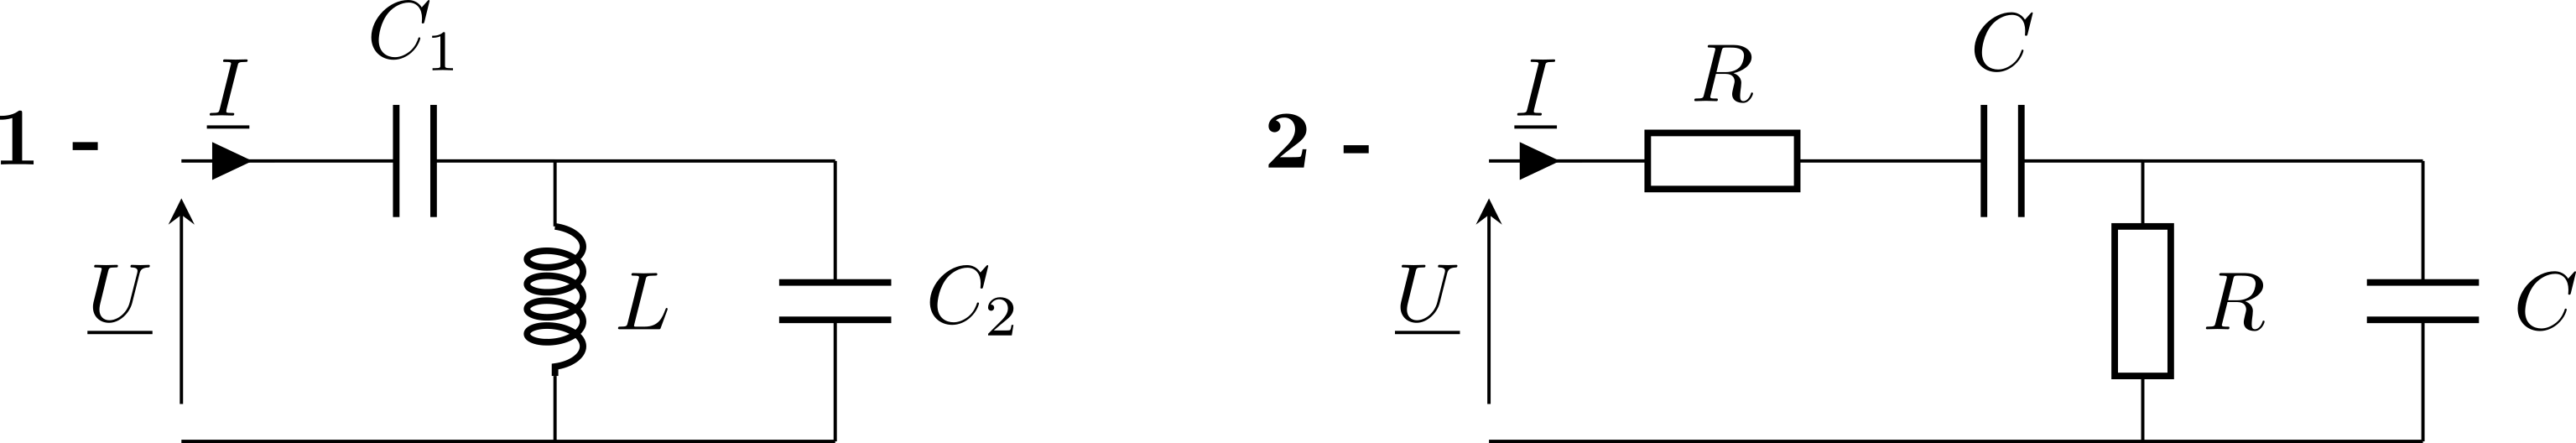
\includegraphics[width=.8\linewidth]{exo1_plain}
		\end{center}
		\begin{answ}%
			\begin{enumerate}
				\item On commence par convertir le circuit avec les impédances complexes~:
				      \begin{itemize}
					      \item $\Zu_{C_1} = \frac{1}{\jj C_1\w}$~;
					      \item $\Zu_L = \jj L\w$~;
					      \item $\Zu_{C_2} = \frac{1}{\jj C_2\w}$.
				      \end{itemize}
				      On peut ensuite déterminer l'impédance équivalente à l'association
				      en parallèle de $L$ et $C_2$. Avec les admittances, on a
				      \begin{gather*}
					      \Zu\ind{eq,1}
					      = \frac{1}{\frac{1}{\Zu_{C_2}} + \frac{1}{\Zu_L}}
					      = \frac{1}{\jj C_2\w + \frac{1}{\jj L\w}}
					      = \frac{\jj L\w}{1 - \w^2LC_2}
				      \end{gather*}
				      Il suffit alors de faire l'association en série de $\Zu_{C_1}$
				      et de $\Zu\ind{eq,1}$~:
				      \begin{gather*}
					      \boxed{
						      \Zu\ind{eq} = \frac{1}{\jj C_1\w} + \frac{\jj L\w}{1 - \w^2LC_2}}
				      \end{gather*}
				      Il n'est ici pas nécessaire d'aller plus loin dans le calcul.

				\item Ici, on utilise que $\Zu_R = R$ et comme précédemment, on effectue
				      l'association en parallèle des $R$ et $C$ de droite avant de faire
				      l'association en série de $R$ et $C$ de gauche avec cette impédance
				      équivalente~:
				      \begin{gather*}
					      \Zu\ind{eq, 1}
					      = \frac{1}{\frac{1}{\Zu_1} + \frac{1}{\Zu_C}}
					      = \frac{1}{\frac{1}{R} + \jj C\w}
					      = \frac{R}{1 + \jrcw}
				      \end{gather*}
				      Et on a donc finalement
				      \begin{gather*}
					      \boxed{
						      \Zu\ind{eq} = R + \frac{1}{\jj C\w} + \frac{R}{1 + \jrcw}}
				      \end{gather*}
			\end{enumerate}
		\end{answ}%
	}{ % énoncé uniquement
		Déterminer l'impédance complexe équivalente de chacun des dipôles ci-dessous
		en RSF.
		\begin{center}
			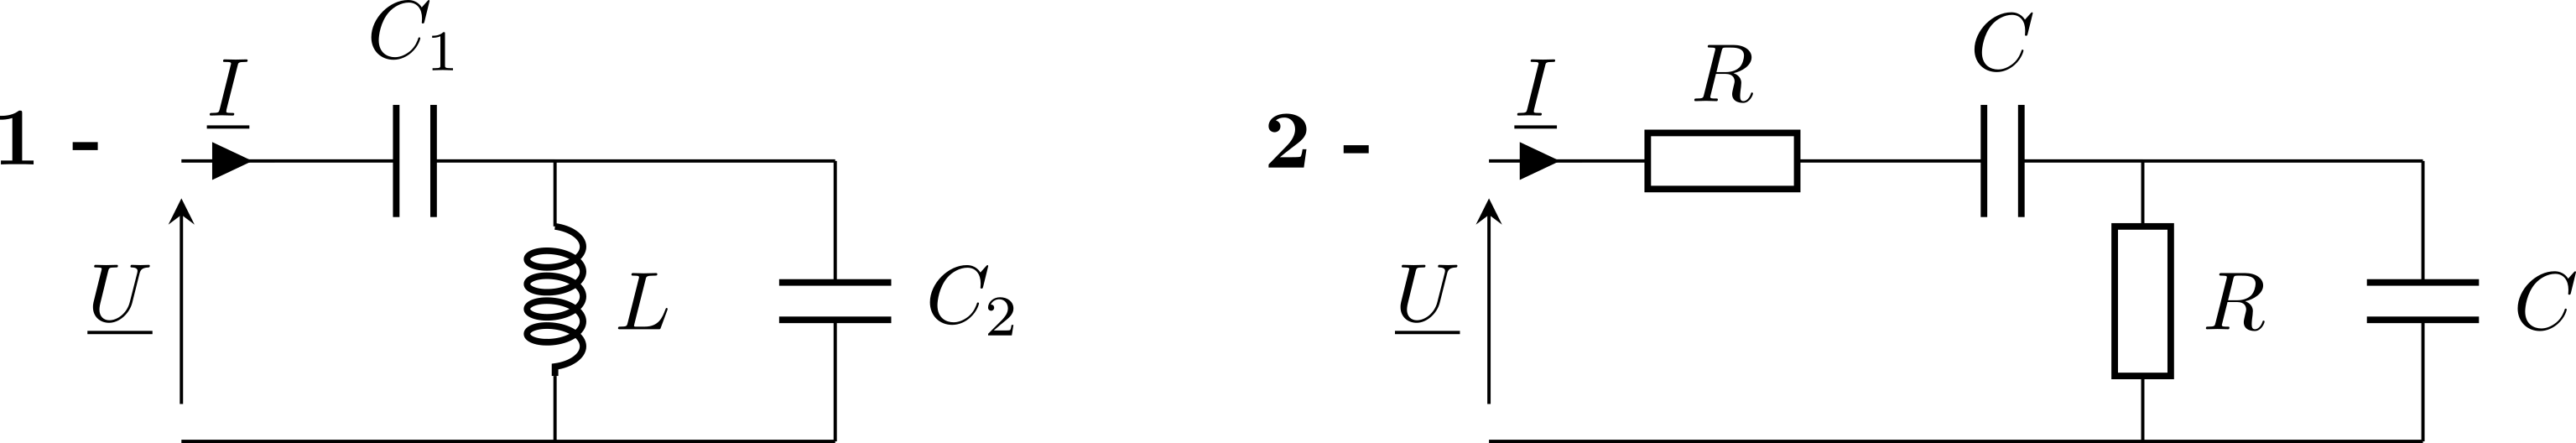
\includegraphics[width=.8\linewidth]{exo1_plain}
		\end{center}
	}
}

\resetQ
\section{Circuit RL série en RSF}
\enonce{%
	\noindent
	\begin{minipage}[t]{.6\linewidth}
		On considère le circuit ci-contre en régime sinusoïdal forcé, où la source de
		tension impose $e(t) = E\cos(\wt)$ avec $E > 0$.
	\end{minipage}
	\hfill
	\begin{minipage}{0.35\linewidth}
		\begin{center}
			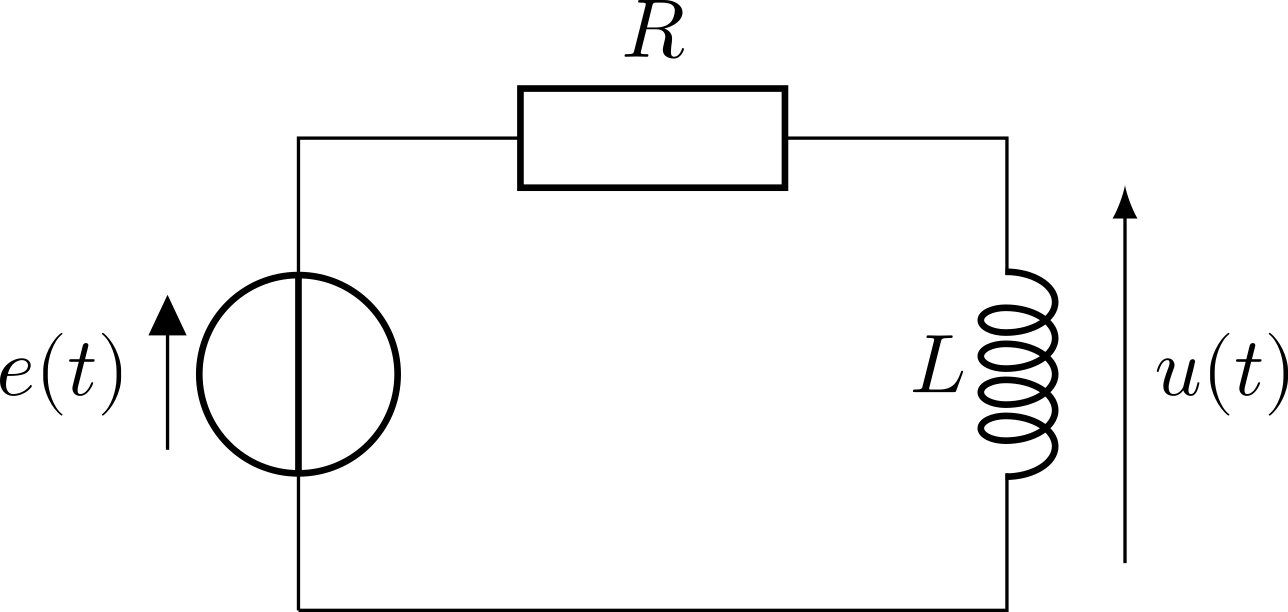
\includegraphics[width=\linewidth]{exo2_plain}
		\end{center}
	\end{minipage}
}

\QR{%
	Déterminer l'amplitude de $u$ à «~très haute~» ($\w\ra\infty$)
	et «~très basse~» ($\w\ra0$) fréquence.
}{%
	Pour les comportements limites, on utilise la modélisation d'une
	bobine à haute et basse fréquence~: étant donné que $\Zu_L = \jj L
		\w$, pour $\w\ra0$ on a $\Zu_L = 0$, et pour
	$\w\ra\infty$ on a $\Zu_L \ra \infty$. On a donc
	respectivement un fil et un interrupteur ouvert. En effet, l'impédance
	étant homogène à une résistance, une impédance nulle est semblable à une
	résistance nulle (un fil), et une impédance infinie est semblable à une
	résistance infinie (un interrupteur ouvert). \bigbreak
	Or, la tension d'un fil est nul, donc
	\[\boxed{u \xrightarrow[\w\ra0]{} 0}\]
	Le courant ne peut traverser un interrupteur, donc en faisant la loi des
	mailles dans le circuit équivalent, on a $u_R = Ri = 0$, et forcément
	\[\boxed{u \xrightarrow[\w\ra\infty]{} E}\]
}

\QR{%
	Exprimer l'amplitude complexe $\Uu$ de $u(t)$ en fonction de $E$,
	$R$, $L$ et $\w$.
}{%
	Pour cela, on utilise la relation du pont diviseur de tension~:
	\begin{gather*}
		\Uu
		= \frac{\Zu_L}{\Zu_L + \Zu_R}E
		\Lra
		\boxed{\Uu
			= \frac{\jj L\w}{R + \jj L \w}E}
	\end{gather*}
}

\QR{%
	Les tensions $e$ et $u$ peuvent-elles être en phase~? En opposition de
	phase~? En quadrature de phase~? Préciser le cas échéant pour quelle(s)
	pulsation(s).
}{%
	La phase de $e(t)$ est nulle par construction. On calcule donc la
	phase de $u$ en prenant l'argument de son amplitude complexe~:

	\begin{gather*}
		\arg(\Uu)
		= \arg(\jj L\w E) - \arg(R + \jj L \w)
		= \frac{\pi}{2} - \arctan \left( \frac{L\w}{R} \right)
	\end{gather*}
	où on peut prendre l'arctangente parce que la partie réelle est
	positive. Ainsi~:
	\begin{enumerate}
		\item Signaux en phase
		      \begin{gather*}
			      \Lra
			      \arg(\Uu) = 0
			      \Lra
			      \arctan \left( \frac{L\w}{R} \right) = \frac{\pi}{2}
			      \Lra
			      \boxed{\w \longrightarrow \infty}
		      \end{gather*}
		      C'est donc mathématiquement possible et physiquement
		      approchable, mais pas rigoureusement.
		\item Signaux en opposition de phase
		      \begin{gather*}
			      \Lra
			      \arg(\Uu) = \pi
			      \Lra
			      \arctan \left( \frac{L\w}{R} \right) = -\frac{\pi}{2}
			      \Lra
			      \boxed{\w \longrightarrow -\infty}
		      \end{gather*}
		      C'est donc mathématiquement possible, mais \textbf{physiquement
			      impossible}~: la pulsation est proportionnelle à la fréquence,
		      et une fréquence ne saurait être négative.
		\item Signaux en quadrature de phase
		      \begin{gather*}
			      \Lra
			      \arg(\Uu) = \frac{\pi}{2}
			      \Lra
			      \arctan \left( \frac{L\w}{R} \right) = 0
			      \Lra
			      \boxed{\w = 0}
		      \end{gather*}
		      C'est donc possible à la fois mathématiquement et physiquement,
		      mais cela correspond à un signal d'entrée qui ne varie pas,
		      c'est-à-dire un régime permanent~: la sortie n'oscille donc pas
		      non plus, et est simplement nulle. La quadrature de phase n'a
		      donc pas vraiment de sens ici, la sortie est constamment nulle
		      quand l'entrée est à son maximum.
	\end{enumerate}
}

\resetQ
\section{Exploitation d'un oscillogramme en RSF}
\enonce{%
	On considère le circuit ci-dessous. On pose $e(t) = E_m\cos(\wt)$ et $u(t) =
		U_m\cos(\wt+\f)$. La figure ci-dessous représente un oscillogramme réalisé à la
	fréquence $f = \SI{1.2e3}{Hz}$, avec $R = \SI{1.0}{k\Omega}$ et $C =
		\SI{0.10}{\micro F}$.
	\begin{center}
		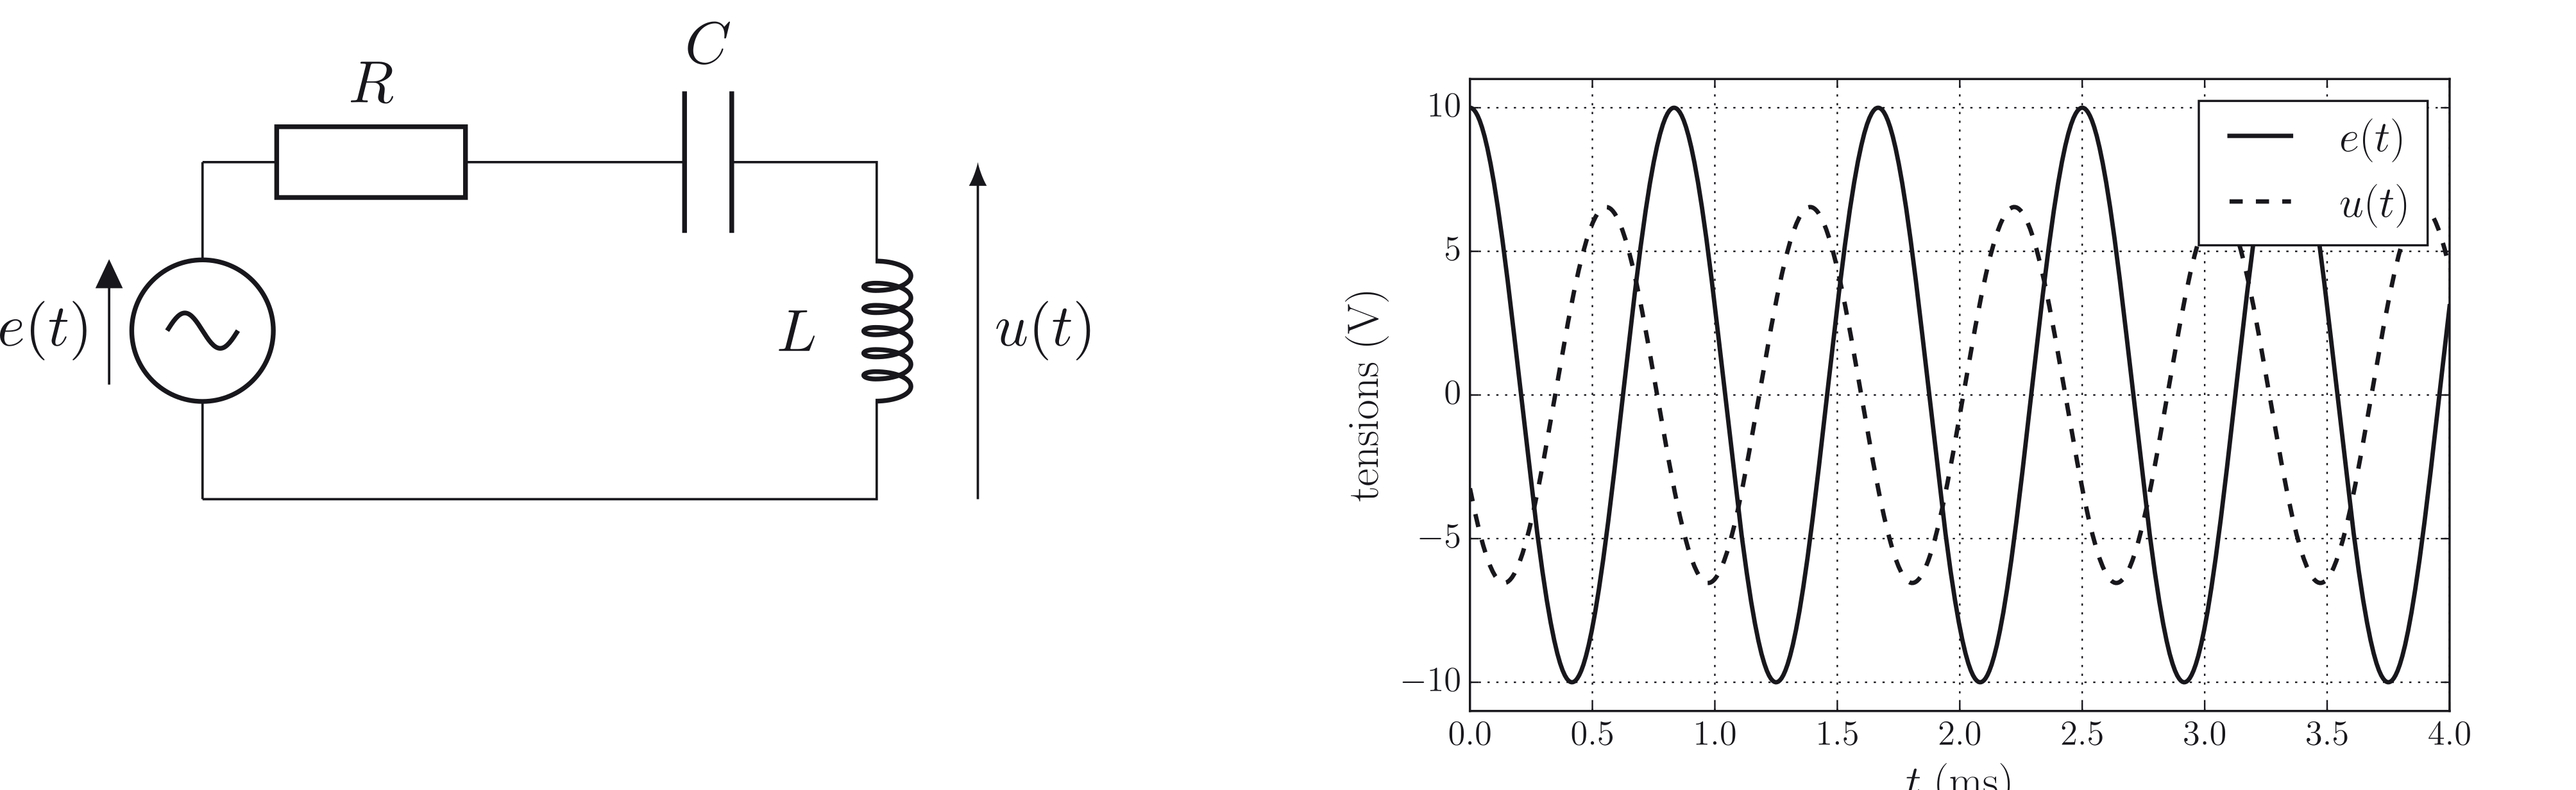
\includegraphics[width=\linewidth]{exo3_plain}
	\end{center}
}
\QR{%
	Déduire de cet oscillogramme les valeurs expérimentales de $E_m$,
	$U_m$ et $\f$.
}{%
	On lit l'amplitude de $e(t)$ à son maximum pour avoir \fbox{$E_m =
			\SI{10}{V}$}. On lit l'amplitude de $u(t)$ à son maximum pour avoir
	\fbox{$U_m = \SI{6}{V}$}. Pour la phase \textbf{à l'origine des temps},
	on regarde le signal à $t = 0$~: on lit $u(0) = U_m\cos(\f) =
		\SI{-3}{V}$, soit
	\begin{gather*}
		\boxed{\cos(\f) = \frac{u(0)}{U_m}}
		\qavec
		\left\{
		\begin{array}{rcl}
			u(0) & = & \SI{-3}{V} \\
			U_m  & = & \SI{6}{V}
		\end{array}
		\right.\\
		\mathrm{A.N.~:}\quad
		\boxed{\f = \frac{2\pi}{3}\si{rad}}
	\end{gather*}
}

\QR{%
	Exprimer $U_m$ et $\f$ en fonction des composants du circuit.
}{%
	On utilise un pont diviseur de tension pour avoir l'amplitude
	complexe~:
	\begin{gather*}
		\Uu
		= \frac{\Zu_L}{\Zu_R + \Zu_C + \Zu_L}E_m
		= \frac{1}{\frac{\Zu_R}{\Zu_L} + \frac{\Zu_C}{\Zu_L}
			+ \frac{\Zu_L}{\Zu_L}}E_m
		\Lra
		\Uu
		= \frac{1}{1 + \frac{R}{\jj L\w} + \frac{1}{\jj^2\w^2CL}}E_m\\
		\Lra
		\boxed{
			\Uu
			= \frac{1}{1 -\jj \frac{R}{L\w} - \frac{1}{\w^2LC}}E_m
		}
	\end{gather*}
	On peut en vérifier l'homogénéité en se souvenant des résultats des
	chapitres précédents~:
	\begin{gather*}
		\w_0{}^2 = \frac{1}{LC}
		\qdonc
		\w^2LC \text{ adimensionné}
		\qet
		\frac{R}{L} = \tau^{-1}
		\qdonc
		\frac{R}{L\w} \text{ adimensionné}
	\end{gather*}
	D'une manière générale, on exprimera les résultats de la sorte, avec une
	fraction dont le numérateur est homogène à la quantité exprimée alors
	que le dénominateur est adimensionné. \bigbreak
	On trouve l'amplitude réelle en prenant le module de cette expression~:
	\begin{gather*}
		U_m
		= \abs{ \Uu }
		\Lra
		\boxed{U_m
			= \frac{E}{\sqrt{\left(1 - \frac{1}{LC\w^2}\right)^2 +
					\frac{R^2}{L^2\w^2}}}
		}
	\end{gather*}
	On trouve la phase en en prenant l'argument~:
	\begin{gather*}
		\f
		= \arg(\Uu)
		= \underbrace{\cancel{\arg(E)}}_{=0}
		- \arg \left( 1 - \frac{1}{LC\w^2} - \jj \frac{R}{L\w}
		\right)\\
		\Lra
		\tan(\f)
		= - \left(-\frac{R}{L\w}\times \frac{1}{1 - \frac{1}{LC\w^2}}\right)
		= \frac{R}{L\w - \frac{1}{C\w}}
		\Lra
		\boxed{\tan(\f)
			= \frac{RC\w}{LC\w^2 - 1}
		}
	\end{gather*}
	Ici, il n'est pas évident de prendre l'arctangente de la tangente~: la
	partie réelle de l'argument calculé n'est pas forcément positif (il
	l'est si $\w^2 > \frac{1}{LC}$).
}

\QR{%
	En déduire la valeur numérique de l'inductance $L$ de la bobine.
}{%
	Il paraît évidemment plus simple de calculer $L$ à partir de la phase,
	sachant qu'on a déterminé $\f$ à la première question~:
	\begin{gather*}
		LC\w^2 - 1
		= \frac{RC\w}{\tan(\f)}
		\Lra
		LC\w^2 = 1 + \frac{RC\w}{\tan(\f)}\\
		\Lra
		\boxed{L = \frac{1}{C\w^2} + \frac{R}{\w\tan(\f)}}
		\qavec
		\left\{
		\begin{array}{rcl}
			C  & = & \SI{0.10}{\micro F}    \\
			\w & = & 2\pi f                 \\
			f  & = & \SI{1.2e3}{Hz}         \\
			R  & = & \SI{1}{k\Omega}        \\
			\f & = & \frac{2\pi}{3}\si{rad}
		\end{array}
		\right.\\
		\mathrm{A.N.~:}\quad
		\boxed{L = \SI{9.9e-2}{H}}
	\end{gather*}
}

\resetQ
\section{Comportement d'un circuit à haute et basse fréquence}
\enonce{%
	\noindent
	\begin{minipage}[t]{.6\linewidth}
		On considère le circuit ci-contre. On pose $e(t) = E_m\cos(\wt)$ et $u(t) =
			U_m\cos(\wt+\f)$.
	\end{minipage}
	\hfill
	\begin{minipage}{0.35\linewidth}
		\begin{center}
			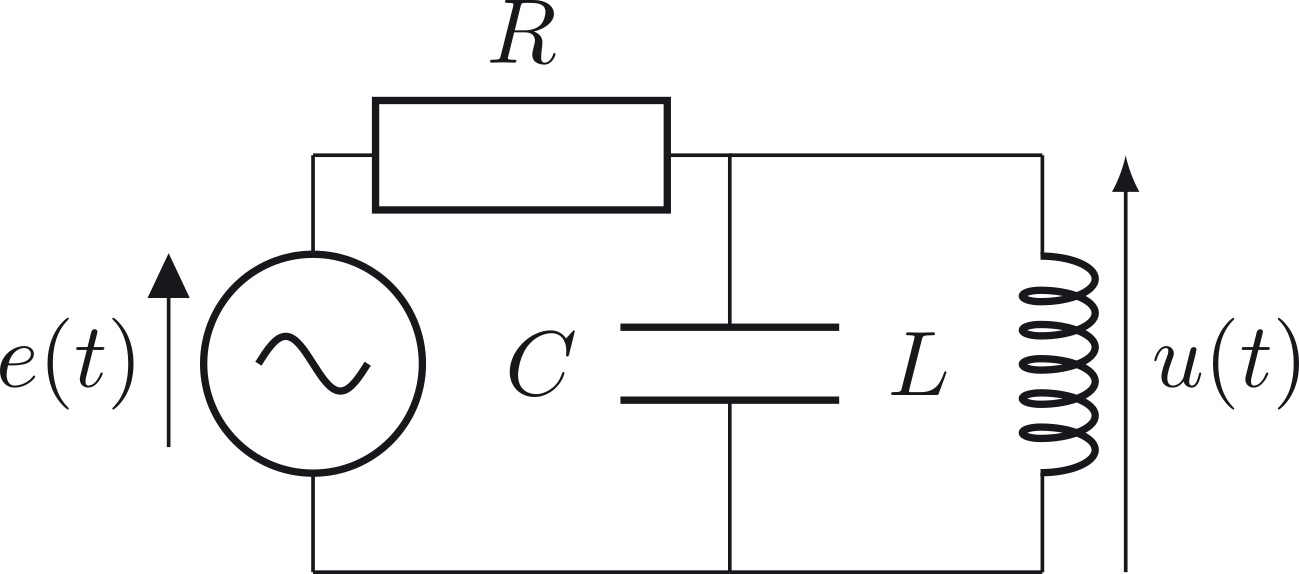
\includegraphics[width=\linewidth]{exo4_plain}
		\end{center}
	\end{minipage}
}

\QR{%
	Définir les signaux complexes $\xul{e}(t)$ et $\xul{u}(t)$ puis les
	amplitudes complexes $\Eu$ et $\Uu$ associées aux tensions
	$e(t)$ et $u(t)$, respectivement.
}{%
	On utilise la relation pour passer des réels aux complexes, pour avoir
	\[
		\boxed{\xul{e}(t) = E_m\exr^{\jwt}}
		\qet
		\boxed{\xul{u}(t) = U_m\exr^{\jj(\wt+\f)}}
	\]
	Pour avoir les amplitudes complexes, on sépare le terme en $\wt$ du
	terme de phase~: on trouve donc
	\[
		\boxed{\Eu = E_m}
		\qet
		\boxed{\Uu = U_m\exr^{\jj\f}}
	\]
}

\QR{%
	Établir l'expression de $\Uu$ en fonction de $E_m$, $R$, $L$,
	$C$ et $\w$.
}{%

	S'il n'y avait pas la capacité, on pourrait facilement utiliser un pont
	diviseur de tension pour exprimer $\xul{u}$ en fonction de $\xul{e}$,
	$\Zu_R$ et $\Zu_L$. Pour se ramener à la situation du pont diviseur de
	tension, on détermine donc une première impédance équivalente issue de
	l'association en parallèle de $L$ et $C$, après les avoir converties en
	complexes. \bigbreak
	On peut déterminer $\Zu\ind{eq, 1}$ avec les admittances $\Yu_L = 1/\jj
		L \w$ et $\Yu_C = \jj C\w$, et utiliser le pont diviseur de tension
	directement avec l'amplitude complexe~: $\Uu =
		\frac{\Zu\ind{eq,1}}{\Zu\ind{eq,1}+\Zu_R}E_m$. Ainsi,
	\begin{gather*}
		\Uu = \frac{\dfrac{1}{
				\color{orange}\cancel{\dfrac{1}{\jj L\w} + \jj C\w}}}
		{\dfrac{1}{\textcolor{orange}{\cancel{\dfrac{1}{\jj L\w} + \jj C\w}}}
			+ R\color{orange}(…)}E_0
		\times \textcolor{orange}{
			\frac{\jj C\w + \dfrac{1}{\jj L\w}}{\jj C\w + \dfrac{1}{\jj L\w}}}
		\Lra
		\Uu = \frac{1}{1 + \jrcw + \dfrac{R}{\jj L\w}}E_0\\
		\Lra
		\boxed{
			\Uu = \frac{E_0}{1 + \jj \left( RC\w - \dfrac{R}{L\w} \right)}
		}
	\end{gather*}
	où on a simplifié la fraction en multipliant par le terme orange d'abord,
	puis en utilisant que $1/\jj = -\jj$.
}

\QR{%
	En déduire les expressions de $U_m$ et de $\f$ en fonction de
	$E_m$, $R$, $L$, $C$ et $\w$.
}{%
	On trouve l'amplitude réelle en prenant le module de l'amplitude
	complexe, et la phase en en prenant l'argument~:
	\begin{gather*}
		U_m
		= \abs{ \Uu }
		\Lra
		\boxed{U_m
			= \frac{E_m}{\sqrt{1 + \left( RC\w - \dfrac{R}{L\w} \right)^2}}
		}\\
		\f
		= \underbrace{\cancel{\arg(E_m)}}_{=0}
		- \arg \left( 1 + \jj \left( RC\w - \dfrac{R}{L\w} \right) \right)
		\Lra
		\tan\f = - \frac{RC\w - \dfrac{R}{L\w}}{1}\\
		\Lra
		\boxed{\f = \arctan \left( RC\w - \frac{R}{L\w} \right)}
	\end{gather*}
}

\QR{%
	Déterminer les valeurs limites de $U_m$ à très basse et très haute
	fréquence. Ces résultats étaient-ils prévisibles par une analyse
	qualitative du montage~?
}{%
	À très haute fréquence, i.e.\ $\w\ra\infty$, le dénominateur
	de l'amplitude réelle tend vers l'infini à cause du terme $RC\w$, donc
	l'amplitude vers 0~; c'est la même chose à très basse fréquence, i.e.\
	$\w\ra0^+$~: le dénominateur tend vers l'infini et l'amplitude
	vers 0, mais cette fois à cause du terme en $\dfrac{R}{L\w}$. On a donc
	\[
		\boxed{U_m \xrightarrow[\w\ra\infty]{} 0}
		\qet
		\boxed{U_m \xrightarrow[\w\ra0^+]{} 0}
	\]
	On pouvait prévoir ces résultats par l'étude directe du montage et des
	impédances en jeu~: en effet,
	\begin{align*}
		\Zu_C
		= \frac{1}{\jj C\w}
		\ra
		\abs{\Zu_C} \xrightarrow[\w\ra0]{} \infty
		 & \qet
		\abs{\Zu_C} \xrightarrow[\w\ra\infty]{} 0 \\
		\Zu_L
		= \jj L\w
		\ra
		\abs{\Zu_L} \xrightarrow[\w\ra0]{} 0
		 & \qet
		\abs{\Zu_L} \xrightarrow[\w\ra\infty]{} \infty
	\end{align*}
	Dans les deux cas, le circuit équivalent est l'association en série
	d'une résistance avec une association en parallèle d'un interrupteur
	ouvert et d'un fil, c'est-à-dire un fil~: or, la tension d'un fil est
	nulle.
}

\resetQ
\section{Dipôle inconnu}

\enonce{%
	\begin{minipage}{0.60\linewidth}
		Dans le montage ci-contre, le GBF délivre une tension $e(t)$ sinusoïdale de
		pulsation $\w$, $R$ est une résistance et $D$ un dipôle inconnu. On note
		$u(t) = U_m\cos(\wt)$ et $v(t) = V_m\cos(\wt+\F)$ les tensions aux bornes
		respectivement de $R$ et $D$. On visualise à l'oscilloscope $v(t)$ et
		$u(t)$, et on obtient le graphe ci-dessous.
	\end{minipage}
	\begin{minipage}{0.35\linewidth}
		\begin{center}
			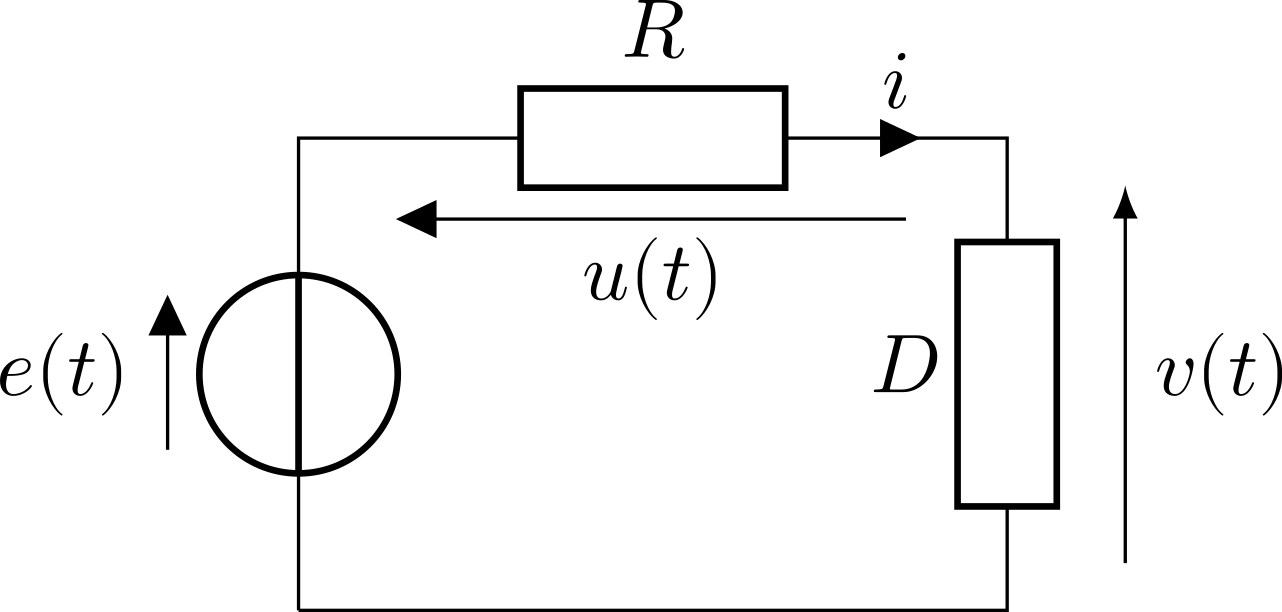
\includegraphics[width=\linewidth]{exo5_plain}
		\end{center}
	\end{minipage}

	\begin{center}
		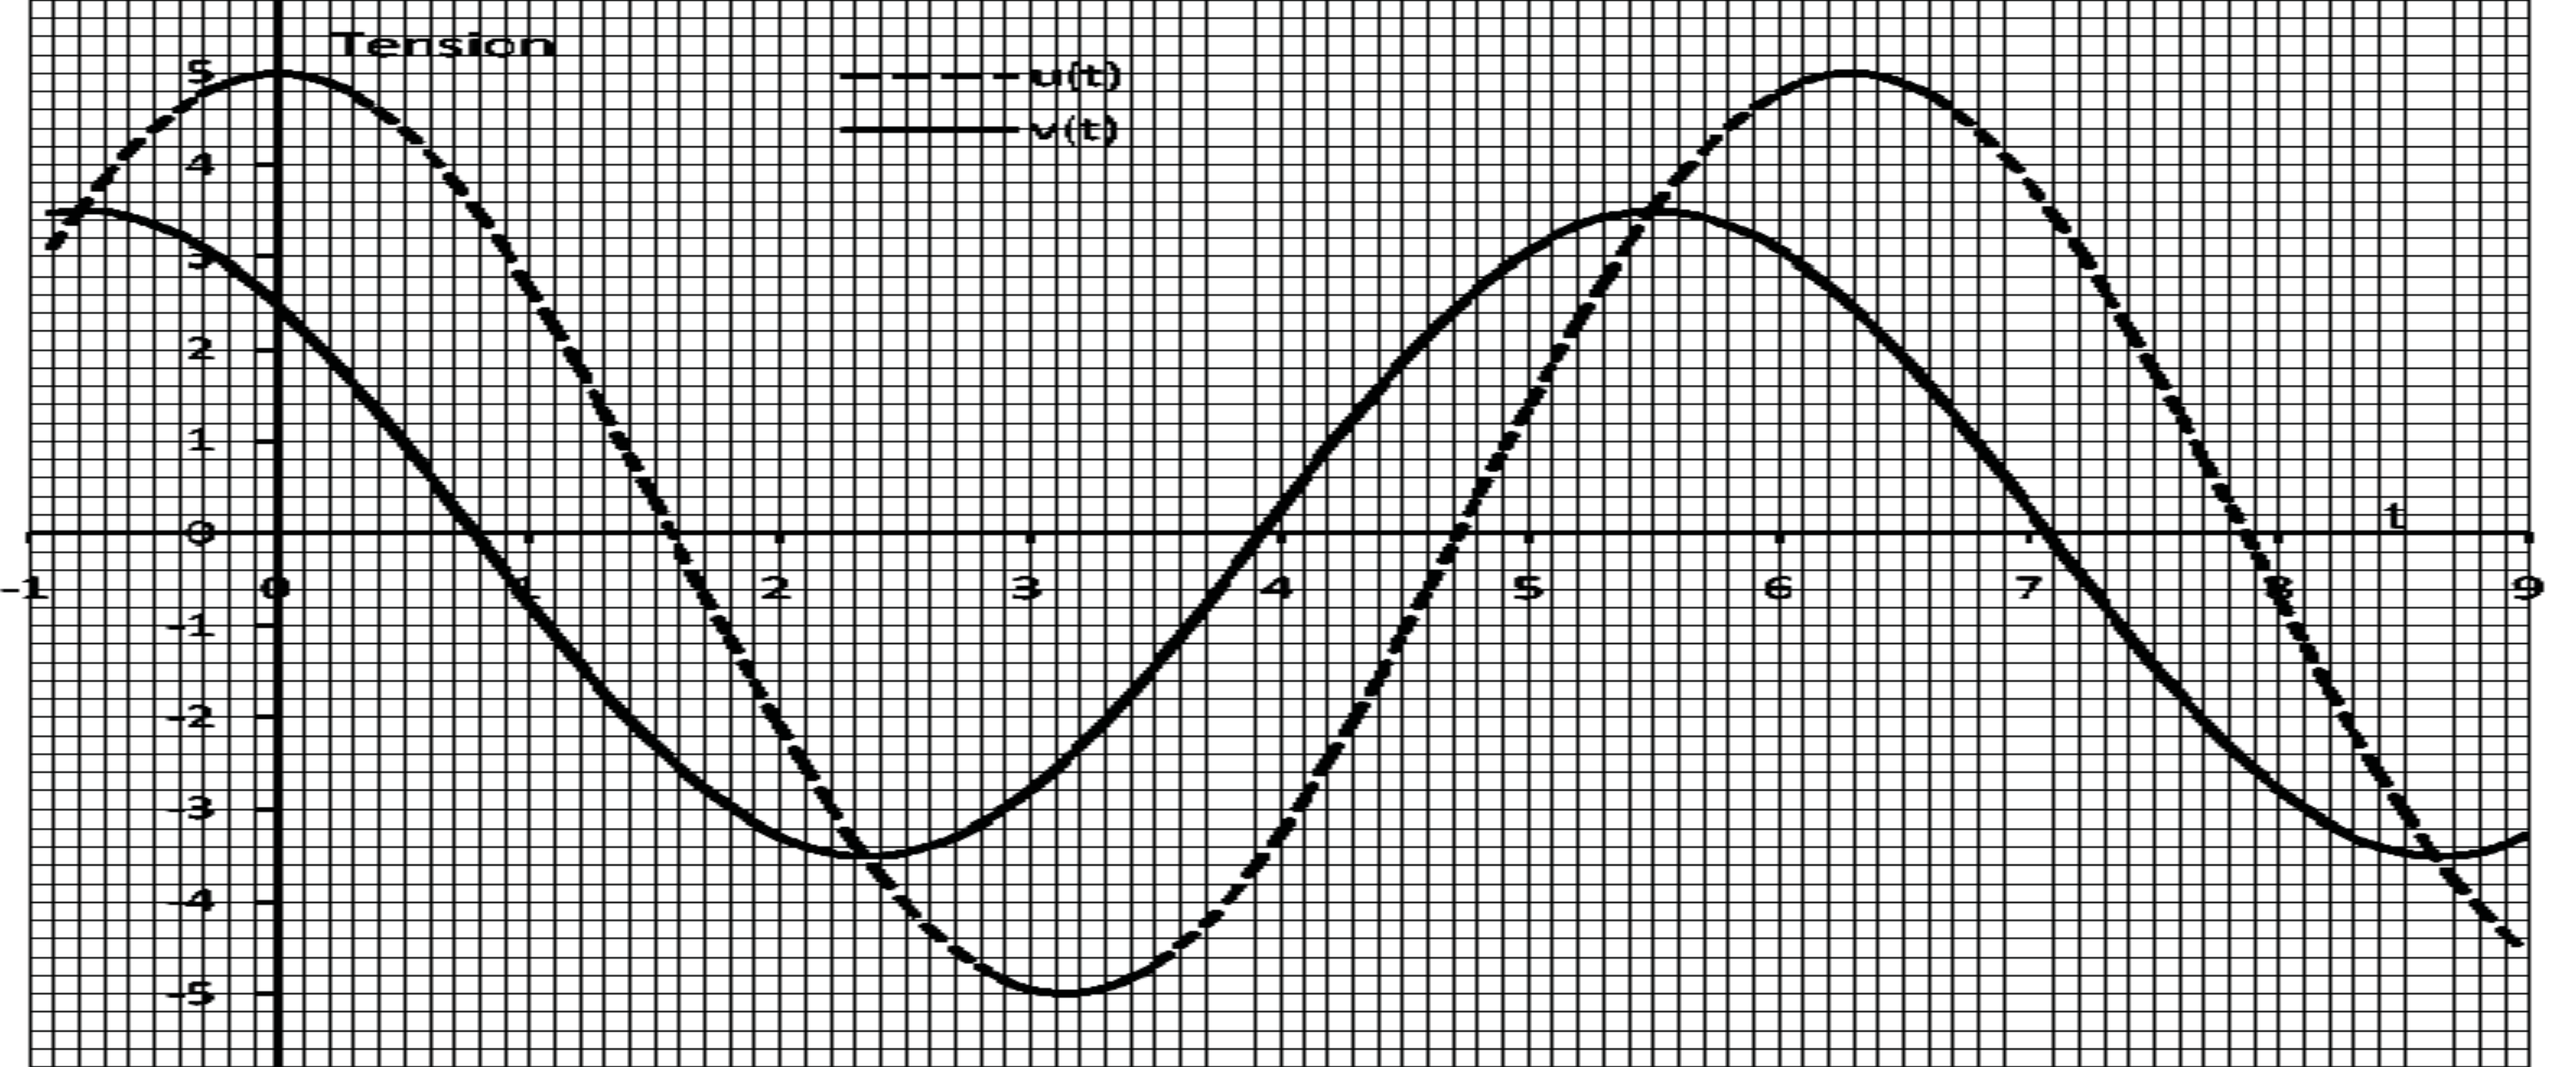
\includegraphics[width=\linewidth]{exo5_plain-2}
	\end{center}

	L'unité de l'axe des temps est $\SI{e-2}{s}$, et celle de l'axe des tensions est
	\SI{1}{V}. On utilise ces résultats graphiques pour déterminer les
	caractéristiques de $D$, sachant que $R = \SI{100}{\Omega}$.
}

\QR{%
	Déterminer $V_m$, $U_m$ ainsi que la pulsation $\w$ des signaux
	utilisés.
}{%
	On trouve les amplitudes par lecture graphique des maxima~:
	\[
		\boxed{V_m = \SI{3.5}{V}}
		\qet
		\boxed{U_m = \SI{5}{V}}
	\]
	On fait de même pour trouver la période $T = \SI{6.3e-2}{s}$, et on en
	déduit la pulsation~:
	\[\boxed{\w = \frac{2\pi}{T} = \SI{100}{rad.s^{-1}}}\]
}

\QR{%
	La tension $v$ est-elle en avance ou en retard sur la tension $u$~? En
	déduire le signe de $\F$. Déterminer la valeur de $\F$ à partir du
	graphe.
}{%
	La tension $v$ est en $avance$ sur $u$, puisque quand $v$ s'annule en
	descendant $u$ s'annule aussi en descendant un peu plus tard que $v$. On
	peut aussi voir qu'à $t=0$, $u$ est à son maximum alors que $v$ y est
	déjà passé et est en train de diminuer. Par définition du déphasage, on
	a donc \fbox{$\D\f_{v/u} > 0$}. \bigbreak
	Or, $\D\f_{v/u} = \f_v - \f_u$ et $u(t) = U_m\cos(\wt)$ donc $\f_u = 0$.
	On trouve donc \fbox{$\F > 0$}. \bigbreak
	On a deux manières de mesurer le déphasage~:
	\begin{itemize}
		\item par définition, la pulsation est une vitesse angulaire, donc
		      une durée se convertit en phase en la multipliant par $\w$. On
		      peut donc déterminer le \textbf{déphasage} en mesurant le
		      \textbf{retard temporel} entre les deux signaux \textbf{quand
			      ils s'annulent avec la même pente}. Soit $\D t$ cet écart~: on
		      mesure
		      \begin{gather*}
			      \D t = \SI{0.75e-2}{s}
			      \Lra
			      \D\f_{v/u} = \F = \w\D t
			      \Lra
			      \boxed{\F = \SI{0.75}{rad} \approx \frac{\pi}{4}\si{rad}}
		      \end{gather*}
		\item On peut également mesurer $v(0) = V_m\cos(\F)$ et avoir
		      \begin{gather*}
			      \cos(\F) = \frac{v(0)}{V_m}
			      \Lra
			      \boxed{\F = \arccos \left( \frac{v(0)}{V_m} \right)}
			      \qavec
			      \left\{
			      \begin{array}{rcl}
				      v(0) & = & \SI{2.5}{V} \\
				      V_m  & = & \SI{3.5}{V}
			      \end{array}
			      \right.\\
			      \mathrm{A.N.~:}\quad
			      \boxed{\F \approx \SI{0.77}{rad}}
		      \end{gather*}
	\end{itemize}
}
\begin{blocQR}
	\item On note $\Zu = X + \jj Y$ l'impédance complexe du dipôle $D$.

	\QR{%
		Déterminer les valeurs de $X$ et $Y$ à partir des résultats
		précédents.
	}{%
		On nous donne $v(t)$ donc $\xul{V} = V_m\exr^{\jj\F}$, et on
		nous défini $\Zu$ son impédance. Pour faire le lien entre
		les deux, on utilise la définition de l'impédance complexe pour
		un dipôle de tension $\Uu$ et traversé par un courant
		$\xul{I}$ \textit{via} loi \textbf{loi d'Ohm généralisée}~:
		\[\boxed{\xul{V} = \Zu\xul{I}}\]
		Il faudrait donc pouvoir connaître $\xul{I}$. Heureusement, la
		loi d'\textsc{Ohm} généralisée fonction évidemment avec les
		résistances, et comme il n'y a qu'une seule intensité qui
		traverse la maille, on peut utiliser
		\[\boxed{\Uu = R\xul{I} \Lra \xul{I} =
				\frac{\Uu}{R}}\]
		Ainsi,
		\begin{gather*}
			Z = \abs{ \Zu } = \sqrt{X^2 + Y^2} \qet
			Z = \abs{ \Zu } = \abs{\frac{\xul{V}}{\xul{I}}}
			= \abs{ R\frac{\xul{V}}{\Uu} }\\
			\Lra
			\boxed{X^2 + Y^2 = R^2 \frac{V_m{}^2}{U_m{}^2}}
			\qavec
			\left\{
			\begin{array}{rcl}
				V_m & = & \SI{3.5}{V}      \\
				U_m & = & \SI{5}{V}        \\
				R   & = & \SI{100}{\Omega}
			\end{array}
			\right.\\
			\mathrm{A.N.~:}\quad
			\boxed{X^2 + Y^2 = \SI{4900}{\Omega^2}}
		\end{gather*}
		L'autre équation permettant de résoudre ce système est bien
		évidemment la phase (question 1 puis question 2)~:
		\begin{gather*}
			\tan(\arg(\Zu)) = \frac{Y}{X} \qet \tan(\arg(\Zu)) =
			\tan(\arg(\xul{V}) -
			\underbrace{\cancel{\arg(\Uu)}}_{=0}) = \tan(\F)\\
			\Lra
			\frac{Y}{X} = \tan\F
			\qavec
			\F = \frac{\pi}{4}\si{rad}
			\qsoit
			\boxed{\frac{Y}{X} = 1}
		\end{gather*}
		On combine les deux équations pour trouver
		\begin{gather*}
			Y = X
			\qet
			2X^2 = \SI{3900}{\Omega^2}\\
			\mathrm{A.N.~:}\quad
			\boxed{X = Y = \SI{49}{\Omega}}
		\end{gather*}
	}

	\QR{%
		Par quel dipôle (condensateur, bobine, résistance) peut-on
		modéliser $D$~?
	}{%
		La partie réelle est non nulle, donc on a au moins une
		résistance de $\SI{49}{\Omega}$, et la partie imaginaire est
		positive~: ça ne peut qu'être une inductance car $1/\jj C\w =
			-\jj/C\w$ et la partie imaginaire est donc négative. C'est donc
		\textbf{l'association en série d'une résistance $r$ et d'une
			inductance $L$}. On trouve
		la valeur de $L$ en calculant $L\w = Y = \SI{49}{\Omega}$.
		\[
			\boxed{r = \SI{49}{\Omega}}
			\qet
			\boxed{L = \SI{0.49}{H}}
		\]
	}
\end{blocQR}

\resetQ
\section{Obtention d'une équation différentielle}
\QR{%
	\begin{minipage}[t]{0.60\linewidth}
		En utilisant les complexes, montrer que la tension $u(t)$ est solution de
		l'équation différentielle
		\[4\tau^2 \dv[2]{u}{t} + 5\tau \dv{u}{t} + u(t) = e(t)
			\qavec
			\tau = RC
		\]
	\end{minipage}
	\hfill
	\begin{minipage}[t]{0.35\linewidth}
		\vspace{0pt}
		\begin{center}
			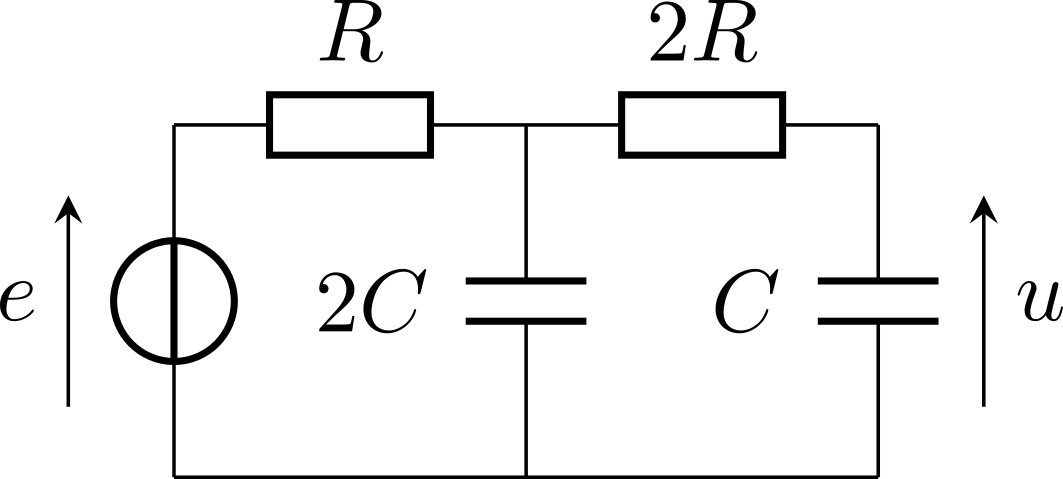
\includegraphics[width=\linewidth]{exo6_plain}
		\end{center}
	\end{minipage}
}{%
	On nomme les tensions et intensités dans le circuit, et on utilise la loi des
	nœuds et la loi d'Ohm généralisée~:

	\begin{minipage}{0.70\linewidth}
		\begin{gather}
			\nonumber
			\xul{I} = \xul{I_1} + \xul{I_2}\\
			\nonumber
			\Lra
			\frac{1}{R}\xul{U_R} = \frac{1}{\Zu_{2C}}\xul{U'} + \frac{1}{\Zu_C}\Uu\\
			\label{eq:ex6}
			\Lra
			\xul{U_R} = 2\jrcw\xul{U'} + \jrcw\Uu
		\end{gather}
	\end{minipage}
	\begin{minipage}{0.30\linewidth}
		\centering
		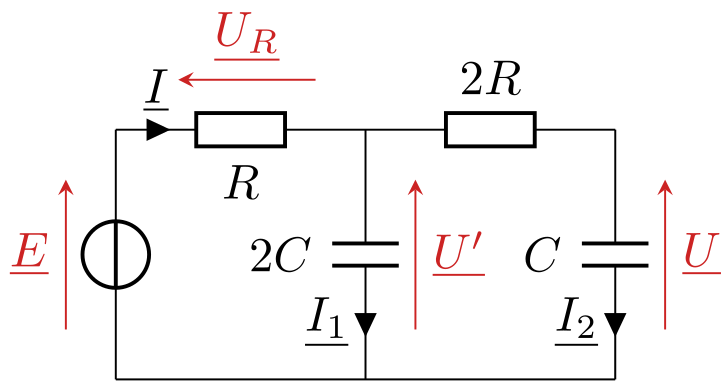
\includegraphics[width=\linewidth]{exo6_solve}
	\end{minipage}
	On utilise ensuite la loi des mailles à droite et à gauche, donnant
	respectivement~:
	\begin{gather*}
		\xul{U'} = \Uu + 2R\xul{I_2} = \Uu + 2\jrcw\Uu
		\qet
		\xul{U_R} = \Eu - \xul{U'} = \Eu - \Uu - 2\jrcw\Uu
	\end{gather*}
	On regroupe les équations dans \eqref{eq:ex6} et on introduit $\tau = RC$~:
	\begin{gather*}
		\Eu - \Uu - 2\jw\tau\Uu = \jw\tau \left( \Uu +
		2\jw\tau\Uu \right) + \jw\tau\Uu\\
		\Lra
		\Eu = \Uu + 5\jw\tau\Uu + 4\tau^2 (\jw)^2\Uu
	\end{gather*}
	En identifiant les puissances de $\jw$ à l'ordre des dérivées pour retourner
	dans le domaine des représentations réelles, on a donc bien
	\begin{gather*}
		\boxed{
			e = u + 5\tau \dv{u}{t} + 4\tau^2 \dv[2]{u}{t}}
	\end{gather*}
	\relax
}

% TODO: Reprendre correction en prenant la partie imaginaire. Cf. rM, notes
% rapides, page 8, tag "todo".

\resetQ
\section{Déphasage, pulsation et impédance}
\QR{%
	\begin{minipage}[t]{0.55\linewidth}
		On considère le circuit ci-contre en RSF. Déterminer l'expression de la
		pulsation $w$ de la tension sinusoïdale $e(t) = E\cos(\wt)$ pour que le
		courant $i(t)$ soit en phase avec $e(t)$.
		\bigbreak
		\textit{Indication}~: utiliser l'impédance équivalente constituée de $C$,
		$L$ et $R_2$.
	\end{minipage}
	\hfill
	\begin{minipage}[t]{0.40\linewidth}
		\vspace{0pt}
		\begin{center}
			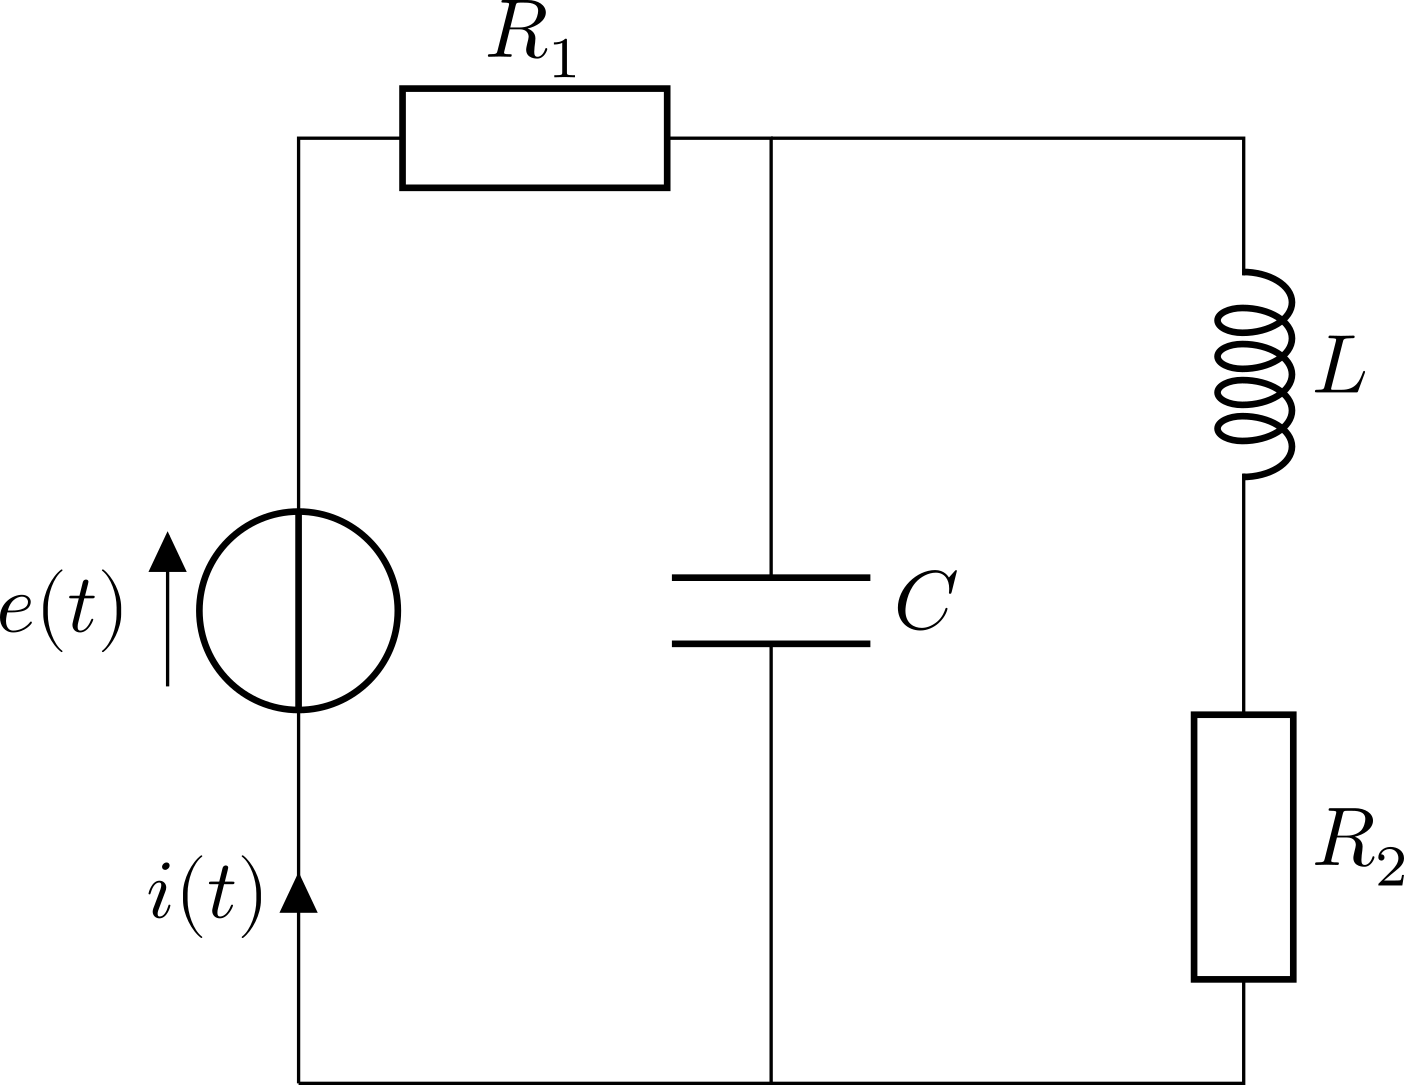
\includegraphics[width=\linewidth]{exo7_plain}
		\end{center}
	\end{minipage}
}{%
	Pour exprimer simplement $i$, il nous faut une seule maille avec une seule
	impédance équivalente $\Zu\ind{eq}$~: de cette manière, la loi des mailles nous
	donnera $\Eu = \Zu\ind{eq}\xul{I}$ et on pourra facilement déterminer le
	déphasage entre $i$ et $e$. \bigbreak
	On calcule l'impédance équivalente de l'association en série de $R_2$ et $L$~:
	\[\Zu\ind{eq,1} = R_2 + \jj L\w\]
	Cette association est en parallèle avec $C$~:
	\begin{gather*}
		\Zu\ind{eq, 2}
		= \frac{\Zu_C\times\Zu\ind{eq, 1}}{\Zu_C + \Zu\ind{eq,1}}
		= \frac{\dfrac{1}{\jj C\w}(R_2 + \jj L\w)}{\dfrac{1}{\jj C\w} + R_2 +
			\jj L\w}\\
		\Lra
		\Zu\ind{eq,2} = \frac{R_2 + \jj L\w}{1+\jj R_2C\w - LC\w^2}
	\end{gather*}
	On a donc comme prévu avec la loi des mailles~:
	\[\boxed{\xul{I} = \frac{\Eu}{R_1 + \Zu\ind{eq,2}}}\]
	L'intensité est en phase avec la tension si $\arg(R_1 + \Zu\ind{eq,2}) = 0$,
	c'est-à-dire si
	\begin{align*}
		\arg\left(R_1 + \frac{R_2 + \jj L\w}{1 + \jj R_2C\w - LC\w^2}\right)
		 & = 0                                                            \\
		\Lra
		\arg \left( \frac{R_1 + \jj R_1R_2C\w - LCR_1\w^2 + R_2 + \jj L\w}
		{1 + \jj R_2 C\w - LC\w^2} \right)
		 & = 0                                                            \\
		\Lra
		\arg \left( (R_1 + R_2 - LCR_1\w^2) + \jj(R_1R_2C\w + L\w) \right)
		 & = \arg \left( (1-LC\w^2) + \jj R_2C\w \right)                  \\
		\Lra
		\tan \left(\arg \left( (R_1 + R_2 - LCR_1\w^2) + \jj(R_1R_2C\w + L\w) \right)\right)
		 & = \tan\left(\arg \left( (1-LC\w^2) + \jj R_2C\w \right)\right) \\
		\Lra
		\frac{R_1R_2C\w + L\w}{R_1 + R_2 - LCR_1\w^2}
		 & = \frac{R_2C\w}{1-LC\w}                                        \\
		\Lra
		\frac{R_1 + \dfrac{L\cancel{\w}}{R_2C\cancel{\w}}}{R_1 + R_2 - LCR_1\w^2}
		 & = \frac{1}{1-LC\w^2}                                           \\
		\Lra
		\left( R_1 + \frac{L}{R_2C} \right) \left( 1-LC\w^2 \right)
		 & = R_1 + R_2 - LCR_1\w^2                                        \\
		\Lra
		\cancel{R_1} - \bcancel{LCR_1\w^2} + \frac{L}{R_2C} - \frac{L^2\w^2}{R_2}
		 & = \cancel{R_1} + R_2 - \bcancel{LCR_1\w^2}                     \\
		\Lra
		L
		 & = R_2{}^2 C + L^2C\w^2                                         \\
		\Lra
		\w^2
		 & = \frac{1}{LC} - \frac{R_2{}^2}{L^2}                           \\
		\Lra
		\Aboxed{\w^2
		 & = \frac{1}{LC} \left( 1 - \frac{R_2{}^2C}{L} \right)}
	\end{align*}
}

\resetQ
\section{Oscillateur à quartz}
\enonce{%
	\begin{minipage}{0.60\linewidth}
		Un quartz piézo-électrique se modélise par un condensateur (de capacité
		$C_0$) placé en parallèle avec un condensateur (de capacité $C$) en série
		avec une inductance $L$. On se place en régime sinusoïdal forcé de pulsation
		$\w$.
	\end{minipage}
	\hfill
	\begin{minipage}{0.35\linewidth}
		\begin{center}
			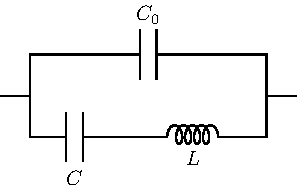
\includegraphics[width=\linewidth]{quartz_plain}
		\end{center}
	\end{minipage}
}

\QR{%
	Donner l'impédance équivalente $\Zu$ de l'oscillateur.
}{%
	On calcule l'association en série de $C$ et $L$ d'abord, puis on fait
	l'association en parallèle de ce dipôle avec $C_0$~:
	\begin{gather*}
		\Zu\ind{eq, 1} = \frac{1}{\jj C\w} + \jj L \w
	\end{gather*}
	D'où
	\begin{align*}
		\Zu
		 & = \frac{1}{\Yu_{C_0} + \Yu\ind{eq, 1}}                         \\
		\Lra
		\Zu
		 & = \frac{1}{\jj C_0\w + \dfrac{1}{\frac{1}{\jj C\w} + \jj L\w}}
		\times
		\frac{\frac{1}{\jj C\w} + \jj L\w}{\frac{1}{\jj C\w} + \jj
		L\w}                                                              \\
		\Lra
		\Zu
		 & = \frac{\frac{1}{\jj C\w} + \jj L\w}{1 + \frac{C_0}{C} -
			LC_0\w^2}
		\times
		\frac{\jj C\w}{\jj C\w}                                           \\
		\Lra
		\Zu
		 & = \frac{1 - LC\w^2}{\jj C\w + \jj C_0\w -\jj LCC_0\w^3}        \\
		\Lra
		\Zu
		 & = -\jj \frac{1 - LC\w^2}{(C+C_0)\w - LCC_0\w^3}                \\
		\Lra
		\Aboxed{\Zu
		 & = \jj \frac{LC\w^2 - 1}{\w\left((C+C_0) - LCC_0\w^2\right)}}
	\end{align*}
}

\QR{%
	Trouver la pulsation pour laquelle l'impédance de l'ensemble est
	nulle, puis celle pour laquelle elle est infinie.
}{%
	L'impédance est nulle si le numérateur est nul, c'est-à-dire
	\[\boxed{\Zu = 0 \Lra \w = \w_0 = \sqrt{\frac{1}{LC}}}\]
	À cette pulsation, assimilable à la pulsation propre d'un circuit RLC
	série, le dipôle est donc équivalent à un fil. On retrouvera ce
	résultat en étudiant la résonance dans le chapitre suivant. \bigbreak
	L'impédance est infinie si le dénominateur est nul, c'est-à-dire
	\[\boxed{\abs{\Zu} \ra \infty \Lra \w = \w_0' =
			\sqrt{\frac{C+C_0}{LCC_0}}}\]
	Cette pulsation serait la pulsation propre d'une bobine $L$ et d'un
	condensateur de capacité $C\ind{eq} = \frac{CC_0}{C+C_0}$, autrement dit
	l'association en série d'un condensateur $C$ et d'un autre condensateur
	$C_0$ (les inverses des capacités s'ajoutent en série). \smallbreak
	À cette pulsation (dite «~de résonance~», cf.\ chapitre suivant), la
	bobine et les condensateurs se chargent et déchargent alternativement,
	l'énergie arrivant dans le dipôle est piégée et n'est pas transmise au
	reste du circuit, comme le fait un interrupteur ouvert.
}

\QR{%
	Tracer l'allure de $\abs{\Zu(\w)}$.
}{%
	\begin{minipage}[t]{0.60\linewidth}
		On regarde les cas limites à très haute et très basse fréquence~:
		\begin{gather*}
			\abs{\Zu} \xrightarrow[\w\ra\infty]{} 0
			\qet
			\abs{\Zu} \xrightarrow[\w\ra0^+]{} \infty
		\end{gather*}
		En effet, à $\w \ra 0$, les condensateurs sont des interrupteurs
		ouverts donc l'impédance totale est celle d'un interrupteur ouvert. À
		l'inverse, à $\w \ra \infty$, les condensateurs sont des fils
		donc l'impédance totale est celle d'un fil~: 0.
	\end{minipage}
	\hfill
	\begin{minipage}[t]{0.45\linewidth}
		\vspace{0pt}
		\begin{center}
			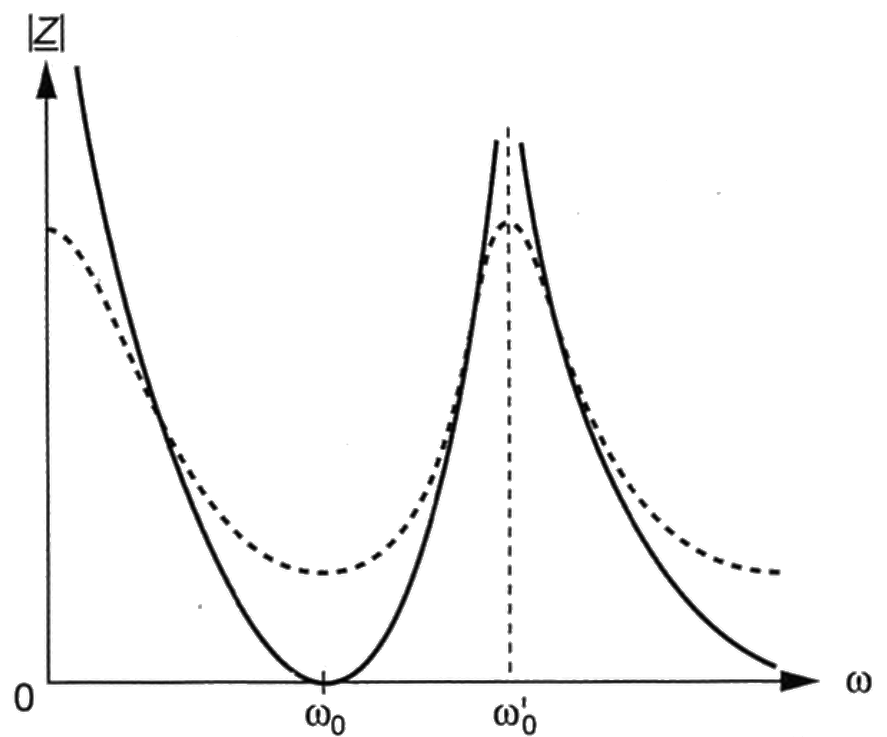
\includegraphics[width=\linewidth]{exo8_solve-clean}
		\end{center}
	\end{minipage}
}

\QR{%
	Comment la courbe précédente serait-elle modifiée si on prenant en
	compte les résistances de chacun des composants~?
}{%
	Les résistances évitent les infinités par dissipation, mais également
	les valeurs nulles~: on se retrouve avec la courbe en pointillés sur la
	figure précédente.
}

\end{document}
